\documentclass{article}

% packages used
\usepackage[utf8]{inputenc}
\usepackage{natbib}
\usepackage{hyperref}
\usepackage{graphicx}

% meta information
\title{Detecting child unsafe videos using transcripts}
\author{Shritishma Reddy \& Pratik Kamble}
\date{February, 17th 2019}

\begin{document}
\maketitle

\section{Abstract}

In this project, we propose an end-to-end pipeline for the detection of child unsafe videos
using video transcripts. Given the spread of digital media and increase in media consumption
by kids (ages 3-12) over the past decade, there is a great need for the filtering of unsafe
content found within reach of said age group. While traditional parental systems do exist,
this would be an online scalable system, that would  only benefit from the increasing video
consumption.

\section{Introduction}

This pipeline has three phases:
\begin{itemize}
    \item{Data acquisition: Collection of a holistic video-transcript dataset representative
    of children viewing habits and trends.}
    \item{Unsafe pattern detection: Analyze speech patterns and clustering hotspot zones to
    form a timeline representation.}
    \item{Video Classification: Classification of videos into unsafe types,
    if unsafe, viz. religious, abusive, drug use, etc.}
\end{itemize}

\subsection{Data Acquisition}

The data acquisition process depends a lot on the type of genre distribution.
A study \citep{childtime} has found that  children consume just over three hours of media,
as of 2015; the numbers having since then gone up further. \\

The time spent with on screen media dramatically increases from the toddler to preschool to
school-age years. Children under two have a screen time average of 53 minutes per day.
This increases to almost two and a half hours per day among two to four year old and almost
three hours for kids in the five to eight year old range. By age eight, 96\% of children have
watched TV, 90\% have used a computer, 81\% have played console video games, and 60\% have
played games or used apps on a portable device. Thus by order of data-source, we should have
a dataset representative mainly of TV show content, followed by YouTube and lastly, game video data. \\

Luckily, all video footage from various sources can be obtained from YouTube, along with transcript
data. TV show snippets, actual online vlog and other consumable media, as well as video game footage
can be found on the streaming platform.

\subsection{Unsafe Pattern Detection}

Once we have the annotated data, we have to run through it and classify according to unsafe-ness. Once
criterion that is of importance is categories that may influence minds may be quite different from ones
for adolescents or adults.

\begin{figure}
    \centering
    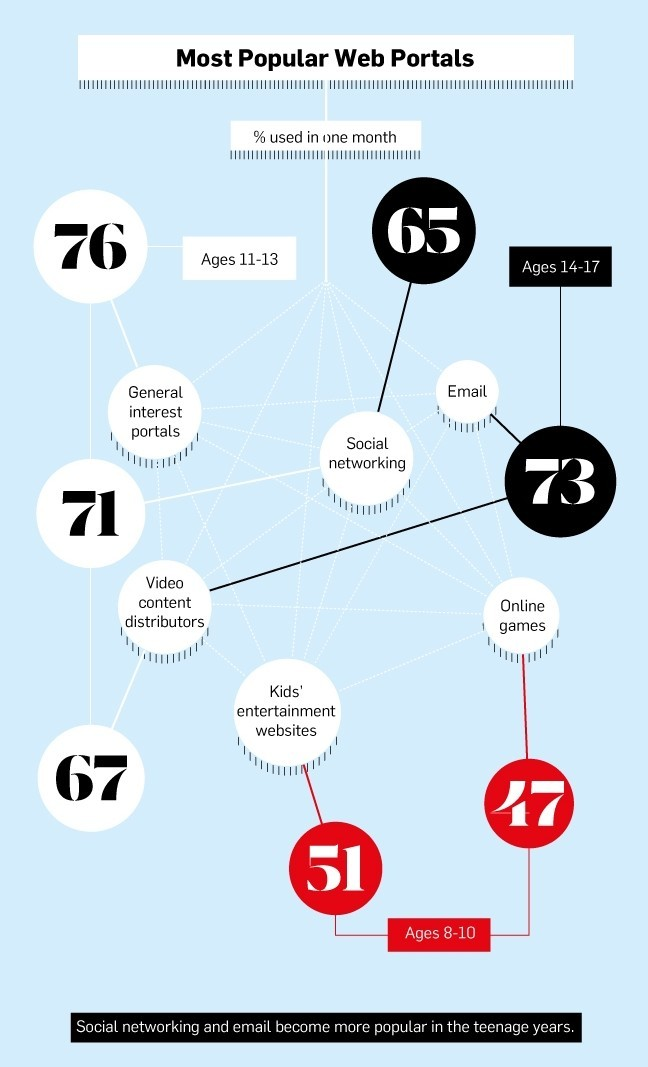
\includegraphics[scale=0.25]{graphic_stats.jpg}
    \caption{Major content sources and distribution}
    \label{fig:genre_dist}
\end{figure}

As seen from the figure \href{fig:genre_dist}, the main categories of media streaming are entertainment
websites, omline games, email, social networking and general interest portals. Breaking down the type of content
found on these sites, the main type of genres are as follows: \\
\begin{itemize}
    \item{Religion-based hate speech: This occurs in chatrooms and online forums, both high target kid influence}
    \item{Color-based hate speech: Depending on race and ethnicity, such sort of speech may be hidden in meaning and
    harder to detect.}
    \item{Foul Language: Kids usually pick up on foul language and the age of such exposure is lower this decade
    than it ever was.}
    \item{Other offensive terminology: Dealing with kids in the lower age bracket, systems need not worry too much about false positives,
    because of the ease of influence of media on early youth.}
\end{itemize}


\subsection{Video Classification}

Once the data collection for the transcripts is done, a simple classical model is used in cascade, to first analyze
and mark scenes and zones in the time frame with dangerous content.\\

This meta information is then passed to a zonal mapping pipeline, that, depending on how many zones of what clusters there are,
estimates a score for each category mentioned prior. Finally, depending on the thresholding for each genre distribution across ages,
a weighted average will judge the videos overall scores.

% Annotation process and ground truth collection
\section{Annotation and labeling}


% Transcript feature extraction - POS/NP tagging to categories
\section{Speech Classification}

% Overall video classification on basis of transcript clustering
\section{Zonal clustering and overall classification}

% Success rate and scalable component
\section{Conclusion}

\bibliographystyle{plain}
\bibliography{references}
\end{document}
